\chapter{Radiodiagn\'ostico anat\'omico estudiado con simulaciones Monte Carlo}

El presente capítulo presenta algunos ejemplos simples del uso de técnicas de simulación Monte Carlo para caracterizar propiedades estructurales de anatomía. Se realizan aplicaciones típicas del ámito de radiodiagnóstico.

\section{Consideraciones para la simulaci\'on de imágenes morf\'ologicas}

Existen diferentes métodos que han sido aplicados e implementados rutinariamente para el imaging médico con la premisa de lograr técnicas no invasivas capaces de prevenir o diagnosticar patologías.

Para el estudio de las tácnicas radiológicas son necesarios conocimientos avanzados de interacción de la radiación ionizante con la materia, específicamente materiales biológicos típicos en pacientes. Desde un punto de vista general, puede caracterizarse a las técnicas de imaging médico según dos categorías: la primera dedicada a extraer información estructural de tipo anatómica y la segunda de carácter funcional para determinar las propiedades metabólicas.

A continuación se presentan métodos numéricos y modelos analíticos, integrados en algoritmos, capaces de modelar los principales fenómenos físicos relacionados con el transporte de radiación y procesos de interacción con medios materiales de interés biológico.

A modo de ejemplo se presentan implementaciones de metodologías conjuntamente con pruebas preliminares para casos de aproximaciones de imaging por contraste de absorción, como radiografía y mamografía.

\section{Radiodiagn\'ostico para estructuras anat\'omicas}

De acuerdo con los capítulos precedentes, los fotones interactuan con las partículas del material irradiado de diferentes maneras y a cada tipo de interacción corresponde funciones de densidad de probabilidad según los modelos de probabilidad para las secciones eficaces de cada tipo de evento.

\begin{figure}
 \centering
 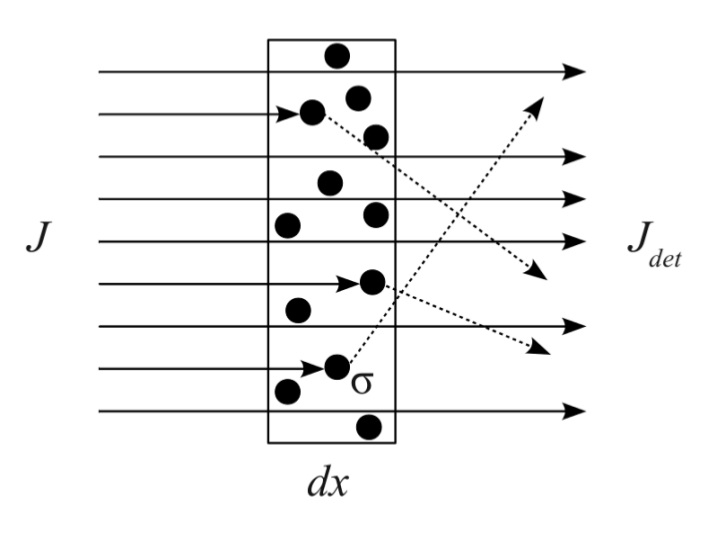
\includegraphics[width = .75\textwidth]{figures/cap8/irrad.png}
 \caption{Esquema de irradiación típico.}
 \label{figirrad}
\end{figure}

Considerando un haz homogéneo de de partículas descrito por la cantidad de partículas por unidad de área por unidad de tiempo ($J = N/ (S \cdot t)$) incidiendo en una muestra delgada de espesor $dx$ de un cierto material, como muestra la figura \ref{figirrad}.

Suponiendo un sistema de detección ideal, colocado para contabilizar sólo partículas que emergen de la muestra irradiada que no hayan interactuado con la muestra.

Resulta que la medición del detector será $J_{det} = J + dJ$, donde $dJ$ indica el número de partículas que efectivamente interactuan con la muestra. Nótese que $dJ$ debe ser una cantidad negativa dado que toma en cuenta las partículas que emergen menos aquellas que inciden en la muestra. 

Debido a que el haz es de distribución espacial uniforme en fluencia en el área de incidencia $S$ y que la muestra delgada puede considerarse, en muy buena aproximación, de características diferenciales $dx$, la fracción de área cubierta por el target resulta que

\begin{equation}
 \frac{dS}{S} = \frac{J - J_{det}}{J} = \frac{-dJ}{J}
\end{equation}

\noindent
donde $dS$ es el área correspondiente a centros de scattering y $S$ es el área total del haz de irradiación.

Si $\sigma$ es la sección eficaz de un único centro de scattering y $dn_{c}$ es el número total de centros de scattering en el volumen $dV$, entonces:

\begin{equation}
 \frac{dS}{S} = \frac{dn_{c} \sigma}{S dx} dx = \frac{dn_{c}}{dV} \sigma dx = \eta \sigma dx \Rightarrow \frac{-dJ}{J} = \eta \sigma dx
\end{equation}

\noindent
donde $\eta \approx dn_{c}/dV$ es el número de centros de scattering por unidad de volumen. En particular, en el caso de un material de densidad $\rho$ y masa molar $M$, $\eta$ se obtiene de:

\begin{equation}
 \eta = \frac{N_{A}\rho}{M}
\end{equation}

\noindent
donde $N_{A}$ es el número de avogadro.

\section{Simulaci\'on Monte Carlo de pr\'acticas de radiograf\'ia y mamograf\'ia}

Los métos de imaging médico generalmente emplean haces externos de rayos X real izando irradiaciones en diferentes modalidades para extraer información estructural. En este sentido, la anatomía de pacientes puede ser obtenida por medio de alguno de estos métodos.

Desde un punto de vista general, las técnicas de imaging médico anatómicas consisten en el uso de haces externos de rayos X generados por Bremsstrahlung y efecto fotoeléctrico de electrones que colisionan con ánodos que constituyen el blanco del tubo de rayos X.

Una vez que la radiación emerge de la muestra después de hacer interactuado con el paciente (o la muestra), se produce la detección por medio de sistemas específicos de detección de radiación, originalmente películas radiográficas, y más recientemente dispositivos como de-
tectores de estado sólido. La detección de la radiación es luego sintetizada para conformar la imagen virtual que puede
plasmarse en formato analógico o digital. 

Por tanto, los principales aspectos y la información requerida para ser incluida en la real-
ización de técnicas de imaging anatómico, son:

\begin{itemize}
 \item Configuración de irradiación especificando la estructura y la disposición geométrica y experimental, así como los componentes instrumentales.
 \item Conocimiento preciso del espectro y características geométricas del haz de radiación incidente.
 \item Información sobre el sistema de detección, como respuesta a la radiación, diseño, calibración, etc.
 \item Anatomía de paciente (o muestra) cuyas propiedades materiales serán inferidas.
 \item Modelos de interacción radiación-materia, los cuales pueden ser obtenidos por medio de modelos teóricos con expresiones analíticas o parámetros tabulados.
\end{itemize}
